% Workflow facts only; technical choice and numerical effects belong in Part II.
\subsection{G3 的可移植复算缺陷触发了真实重建}
离线包没有 Git 目录时，原处理身份代码无法取得 HEAD；相对缓存父目录又在生成仓库内出处时失败。两项实际接口问题分别登记为 G3-C06、G3-C07。B 修复了冻结源码身份的离线校验和路径规范化，没有改变几何、参数或指标定义；C 对新产物独立复验，主线程使受影响的旧版本运行失效并重建。

已有 A 提议和旧结果继续作为历史记录保存；当前决定明确标为在新源码版本下复算，不冒称新的在线模型提议。父任务恢复后才继续条件规则与组合执行。绑定文件、缓存源和审核目标一旦不匹配就拒绝复用，不能只修汇总表而保留失效的决定身份。具体方法裁决与数值在第二层说明。
\subsection{Native 协作证据只按实际可读范围保存}
本轮原生子代理实际参与 A 提案、B 执行与交付、C 独立核验。仅从当前任务 session 导出的工具事件快照截至 2026-09-27 06:54:34.496 UTC，包含 198 个事件、99 次派发或通信调用；后者含 4 次 spawn、34 次 followup 和 61 次 send。这些是工具事件数量，不是底层模型请求数，也不是独立实验次数。本报告绑定此固定时点快照，后续交付与审核事件另存于持续更新的事件索引，不倒写本报告当时的读数。

本地 native message 字段以平台加密值保存，未取得可读逐字原文。工程只导出时间、工具、call ID、可见角色元数据与加密载荷哈希，移除密文正文；没有解密或重建消息。这些哈希不是已知明文的哈希。可读决定另由真实 TaskPlan、执行产物和 C 回执提供，不能称已恢复完整 native 逐字对话。G2 保存的真实 Provider response 与 G1 用户授权原话有各自原始来源，不受这个限制替代或扩充。底层请求和费用仍未知。

\begin{figure}[H]\centering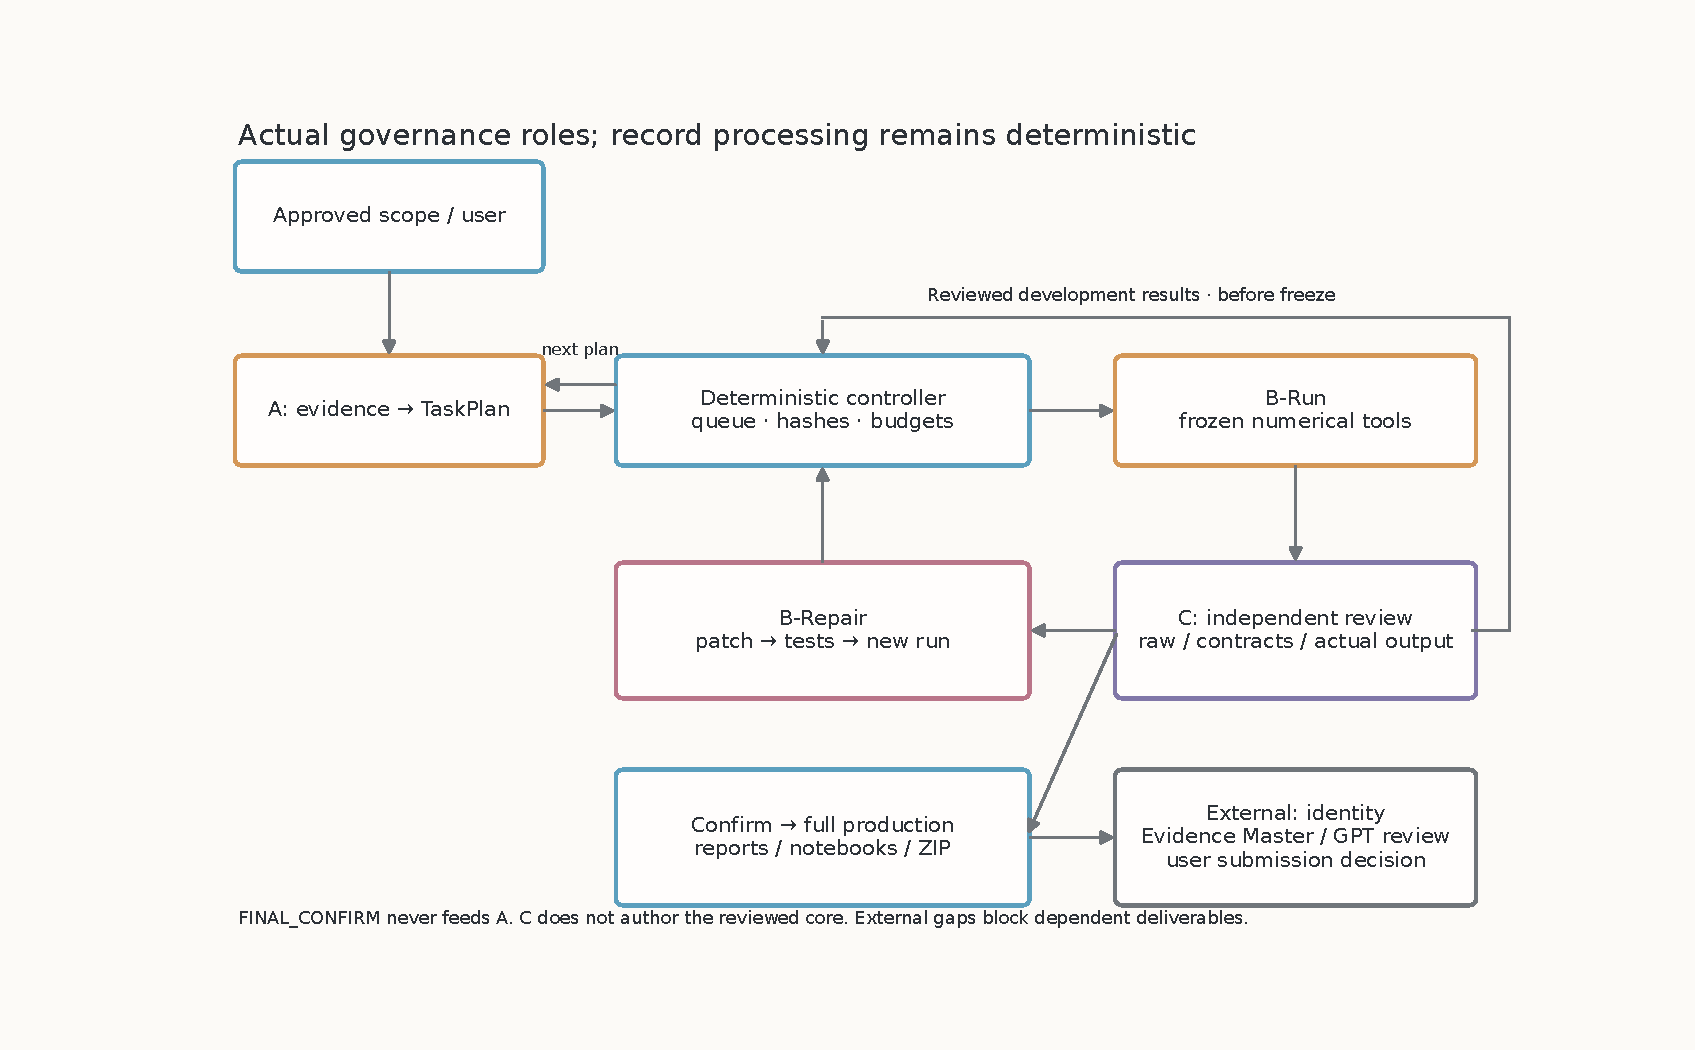
\includegraphics[width=.98\linewidth]{../../figures/goal3/goal3_actual_workflow.pdf}
\caption{本轮实际 A/B/C、确定性控制器、修复返回与外部依赖。角色事件与产物有真实记录；图不代替互动原图或 Evidence Lock。}\end{figure}

